\documentclass{article}
\usepackage{amsmath, amsfonts, amsthm, amssymb, hyperref, titlesec, graphicx, nameref, titling}
\usepackage[utf8]{inputenc}
\usepackage[margin=2cm,heightrounded=true,centering]{geometry}

\DeclareUnicodeCharacter{2009}{\,}

\titleformat{\section}[block]{\color{black}\Large\bfseries}{}{0em}{}[\rule{\linewidth}{1pt}]
\renewcommand\maketitlehooka{\null\mbox{}\vfill} 
\renewcommand\maketitlehookd{\vfill\null}

\title{\Huge{MATLAB:\\ rand vs. randn}}
\author{\huge{Jacob Lyons}}
\date{\Large 7/16/2021}

\hypersetup{colorlinks=true, linkcolor=blue, filecolor=magenta, urlcolor=cyan,}

\newcommand\best[2][Zero]{#1 is the #2 of all time.}
%\newcommand - define a new command being made
%\best - new command name/trigger
%[2] - number of arguements
%[Zero] - default #1 if one isn't given
%{#1 is the #2 of all time.} - command structure.
%use -> \best{input #2} or \best[input #1]{input #2}
%if #1 isn't defined, uses default (in this case is 'Zero')

%\newcommand{<name>}[<args>]{<code>}

\newtheorem{Rules}{Rule}

\newcounter{ex}[section]
\numberwithin{ex}{section}

\newenvironment{Paragraph}[1][]
{
	{\refstepcounter{ex}}
	\begin{flushleft}
		\textbf{\theex}
	\end{flushleft}
}

\begin{document}
	
	\maketitle
	


	\newpage

\section{Normally Distributed Numbers}

	\label{The Greatest invention of all times}
	
	\large What is the difference between uniformly distributed numbers and normally distributed numbers?
	
	\begin{Paragraph}
		Normal Distribution is a probability distribution which peaks out in the middle and gradually decreases towards both ends of axis.  It is also known as gaussian distribution and bell curve because of its bell like shape.
	\end{Paragraph}
	
	\begin{figure}[p] %%%h,t,p is an option that I’ll explain soon.
		\centering %%%should be clear what this does.
		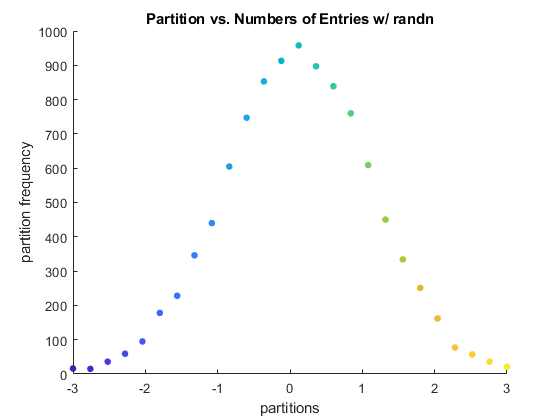
\includegraphics[width=0.5\textwidth]{randn}
		\caption{\label{Coug Logo}This article brought to you by the education of WSU math students!}	
	\end{figure} 

	\begin{Paragraph}
		\noindent The concept of zero as a number arose independently in several different places. In South America, the number system that the Mayans used included a symbol for zero. And the Hindu-Arabic system used throughout most of the world today developed from an earlier Arabic system that used zero as a placeholder. In fact, zero isn’t really nothing — it’s simply a way to express nothing mathematically.
	\end{Paragraph}

\section{Uniformly Distributed Numbers}
	\label{Zero doesn't exist}
	
	\begin{Paragraph}
		In a way, the number zero does not actually exist. The use as a digit is only a placeholder in place value systems. For the simple notion of lacking, the words \textit{nothing} and \textit{none} are often used to explain the concept of zero. Because zero means nothing in math, there is some fallacies that can be created using it as a number. To avoid these, here are a couple rules to always follow when using zero in equations.
		\setcounter{section}{1}
	\end{Paragraph}

	\newpage
	
	
	\begin{Rules}{Do not divide by zero}
		\begin{center}
				
			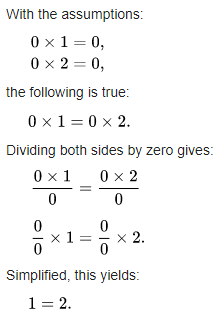
\includegraphics[width=0.3\textwidth]{rule1} \\
			The fallacy here is the assumption that dividing 0 by 0 is a legitimate operation with the same properties as dividing by any other number.	
				
		\end{center}
	\end{Rules}

	\begin{Rules}{You can't do $0^0$}
		\begin{center}
				
			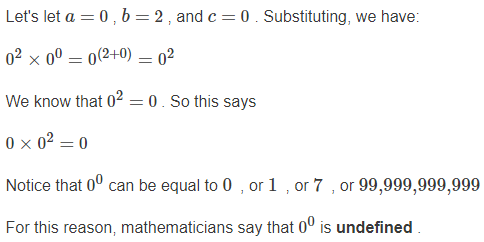
\includegraphics[width=0.6\textwidth]{rule2} \\
			Note: On one hand, any other number to the power of 0 is 1. On the other hand, 0 to the power of anything else is 0. 
			
		\end{center}
	\end{Rules}

	\begin{figure}[p] %%%h,t,p is an option that I’ll explain soon.
		\centering %%%should be clear what this does.
		
\includegraphics[width=0.5\textwidth]{coug}
		\caption{\label{Coug Logo}This article brought to you by the education of WSU math students!}	
	\end{figure} 


\end{document}

